% ============================================================
%  Document d'étude — RL & Projet Airline Dynamic Pricing
%  Compile sur Overleaf (pdfLaTeX), aucun package exotique.
%  Dia Eddine — M2 IADA, Polytech Nice, 2026
% ============================================================
\documentclass[11pt,a4paper]{article}

% ---------- packages standards ----------
\usepackage[utf8]{inputenc}
\usepackage[T1]{fontenc}
\usepackage[french]{babel}
\usepackage{amsmath,amssymb,amsfonts}
\usepackage{booktabs}
\usepackage{array}
\usepackage{enumitem}
\usepackage{geometry}
\usepackage{hyperref}
\usepackage{xcolor}
\usepackage{tcolorbox}
\usepackage{algorithm}
\usepackage{algpseudocode}
\usepackage{tikz}
\usetikzlibrary{arrows.meta, positioning, calc}
\usepackage{graphicx}
\graphicspath{{results/figures/}}
\usepackage{multicol}
\usepackage{fancyhdr}

\geometry{margin=2.2cm}
\hypersetup{colorlinks=true,linkcolor=blue!60!black,urlcolor=blue!60!black}

% ---------- couleurs et boîtes ----------
\definecolor{defblue}{HTML}{2a78d6}
\definecolor{warnred}{HTML}{c0392b}
\definecolor{tipgreen}{HTML}{27ae60}

\newtcolorbox{defbox}[1][]{colback=defblue!5,colframe=defblue!70,
  fonttitle=\bfseries,title=#1}
\newtcolorbox{warnbox}[1][]{colback=warnred!5,colframe=warnred!70,
  fonttitle=\bfseries,title=#1}
\newtcolorbox{tipbox}[1][]{colback=tipgreen!5,colframe=tipgreen!60,
  fonttitle=\bfseries,title=#1}

% ---------- en-tête ----------
\pagestyle{fancy}
\fancyhf{}
\rhead{\small Dia Eddine — M2 IADA 2026}
\lhead{\small RL : guide d'étude}
\rfoot{\thepage}

% ---------- commandes ----------
\newcommand{\E}{\mathbb{E}}
\newcommand{\R}{\mathbb{R}}
\DeclareMathOperator*{\argmax}{argmax}

\title{\textbf{Apprentissage par Renforcement}\\[4pt]
       Guide d'étude \& lien avec le projet\\
       \large\textit{Airline Dynamic Pricing — Plan or Learn?}}
\author{Dia Eddine Kadri — M2 IADA, Polytech Nice}
\date{Octobre 2026}

\begin{document}
\maketitle
\tableofcontents
\newpage

% ============================================================
\section{Le problème en une page}
% ============================================================

\subsection{Le contexte concret}

Une compagnie aérienne vend les billets d'un vol pendant les 30~jours avant le départ. Elle a 10~sièges et 6~prix possibles (50, 80, 110, 140, 170 et 200~€). Chaque jour, elle choisit un prix, des clients arrivent (ou pas), et ceux qui trouvent le prix acceptable achètent.

\begin{itemize}[nosep]
  \item Prix bas $\to$ plus de clients achètent, mais on gagne moins par billet.
  \item Prix haut $\to$ plus de revenu par billet, mais moins de ventes.
  \item L'avion part dans 30~jours \emph{quoi qu'il arrive} : les sièges invendus rapportent 0.
\end{itemize}

\textbf{Objectif :} trouver la stratégie de prix (= politique) qui \textbf{maximise le revenu total}.

\subsection{Pourquoi c'est un problème de RL ?}

\begin{defbox}[Lien avec le cours — session 1]
Le RL s'applique quand on a des \textbf{décisions séquentielles sous incertitude} : ici, chaque jour on choisit un prix (= action), on observe combien de billets sont vendus (= transition stochastique), et on reçoit un revenu (= récompense). Le nombre de clients est aléatoire (loi de Poisson), donc on ne sait pas à l'avance combien on va vendre.

C'est différent du \textbf{supervisé} (pas d'oracle qui dit « le bon prix était 140~€ ») et du \textbf{non supervisé} (on a bien un signal de récompense). $\to$ \textbf{Compétence C1.}
\end{defbox}

\subsection{La question de recherche du projet}

\begin{center}
\fbox{\parbox{0.85\textwidth}{\centering
\textbf{À partir de quelle erreur sur le modèle de demande} devient-il préférable \\
d'\textbf{apprendre sans modèle} (Q-learning / SARSA) \\
plutôt que de \textbf{planifier avec un modèle imparfait} (DP) ?
}}
\end{center}

En clair : la DP a un avantage (elle peut planifier), mais cet avantage disparaît quand son modèle est faux. Le Q-learning, lui, n'a pas de modèle mais apprend par essai-erreur. \textbf{Quand est-ce que l'un dépasse l'autre ?}

% ============================================================
\section{Formalisation en MDP}
\label{sec:mdp}
% ============================================================

\begin{defbox}[Compétences C4, C5]
Un MDP est un tuple $\langle S, A, P, R, \gamma \rangle$ qui modélise un problème de décision séquentielle sous la \textbf{propriété de Markov} : le futur ne dépend que de l'état présent, pas de l'historique.
\end{defbox}

\subsection{Les éléments de notre MDP}

\begin{table}[h]
\centering
\begin{tabular}{@{}lp{10cm}@{}}
\toprule
\textbf{Élément} & \textbf{Dans notre projet} \\
\midrule
\textbf{État} $s = (c, t)$ & $c \in \{0, \ldots, 10\}$ = sièges restants, $t \in \{0, \ldots, 30\}$ = jours restants. \\
& Taille de l'espace d'états : $11 \times 31 = 341$ états. \\
\textbf{Actions} $a$ & Indice du prix : $a \in \{0,1,2,3,4,5\}$ correspondant à $\{50, 80, 110, 140, 170, 200\}$~€. \\
\textbf{Transition} & On tire la demande $d \sim \text{Poisson}(\mu(t, p))$, puis $\text{ventes} = \min(d, c)$. \\
& Nouvel état : $s' = (c - \text{ventes},\ t - 1)$. \\
\textbf{Récompense} & $r = \text{prix}(a) \times \text{ventes}$ (revenu de la journée). \\
\textbf{Fin d'épisode} & $t = 0$ (départ du vol) ou $c = 0$ (avion plein). \\
$\gamma$ & $\gamma = 1$ par défaut (horizon fini). Variante E4 : $\gamma \in \{0.9,\ 0.5\}$. \\
\bottomrule
\end{tabular}
\caption{Notre MDP — chaque ligne correspond à un élément du tuple $\langle S, A, P, R, \gamma \rangle$.}
\end{table}

\subsection{Propriété de Markov dans notre cas (C5)}

L'état $(c, t)$ est-il suffisant pour prédire le futur, sans connaître l'historique ?

\textbf{Oui.} La demande au jour $t$ ne dépend que de $t$ (qui détermine le type de clients) et du prix choisi, pas de ce qui s'est passé les jours précédents. Le nombre de sièges restants $c$ résume parfaitement l'historique des ventes passées.

\subsection{Le modèle de demande}

Deux types de clients, avec des comportements différents :

\begin{table}[h]
\centering
\begin{tabular}{@{}lccc@{}}
\toprule
\textbf{Segment} & \textbf{Arrivées/jour $\lambda(t)$} & \textbf{Quand ?} & \textbf{Prix max accepté (WTP)} \\
\midrule
Loisirs (L) & $\lambda_L = 0{,}8$ si $t > 10$,\ $0{,}3$ sinon & Tôt & Exponentielle, moyenne 80~€ \\
Affaires (B) & $\lambda_B = 0{,}1$ si $t > 10$,\ $1{,}0$ sinon & Tard & Exponentielle, moyenne 180~€ \\
\bottomrule
\end{tabular}
\end{table}

La probabilité qu'un client achète au prix $p$, avec une WTP exponentielle de moyenne $m$ :
\begin{equation}
\boxed{P(\text{achat} \mid p) = e^{-p/m}}
\label{eq:purchase}
\end{equation}
En mots : plus le prix est élevé par rapport à la WTP moyenne, moins le client achète.

Le nombre moyen de ventes (par la propriété d'amincissement de Poisson) :
\begin{equation}
\boxed{\mu(t, p) = \lambda_L(t) \cdot e^{-p/80} + \lambda_B(t) \cdot e^{-p/180}}
\label{eq:demand}
\end{equation}

Et le nombre de ventes du jour : $d \sim \text{Poisson}(\mu(t,p))$, puis $\text{ventes} = \min(d, c)$.

\subsection{Le retour (return) et $\gamma$ (C2, C3)}

Le retour cumulé à partir du pas $t$ :
\begin{equation}
G_t = r_{t+1} + \gamma\, r_{t+2} + \gamma^2 r_{t+3} + \cdots = \sum_{k=0}^{\infty} \gamma^k\, r_{t+k+1}
\end{equation}

\begin{defbox}[Rôle de $\gamma$ — C3]
\begin{itemize}[nosep]
  \item $\gamma = 1$ : toutes les récompenses futures comptent autant $\to$ on maximise le revenu \textbf{total}. C'est notre cas par défaut (horizon fini de 30~jours).
  \item $\gamma = 0$ : seule la récompense immédiate compte $\to$ agent \textbf{myope} qui brade les sièges à bas prix pour vendre tout de suite.
  \item $0 < \gamma < 1$ : compromis. L'expérience E4 montre qu'avec $\gamma = 0{,}5$, la DP vend trop tôt aux clients loisirs et perd les clients affaires qui arrivent tard.
\end{itemize}
\end{defbox}

% ============================================================
\section{Les équations de Bellman}
\label{sec:bellman}
% ============================================================

\begin{defbox}[Compétences C6, C11]
Les fonctions de valeur $V^\pi(s)$ et $Q^\pi(s,a)$ mesurent « combien vaut un état (ou un couple état-action) si on suit la politique $\pi$ ».
\end{defbox}

\subsection{Fonctions de valeur (C6)}

\textbf{Fonction de valeur d'état :}
\begin{equation}
V^\pi(s) = \E_\pi\!\left[G_t \mid s_t = s\right]
\end{equation}
En mots : le revenu moyen qu'on espère obtenir à partir de l'état $s$ en suivant la politique $\pi$.

\textbf{Fonction de valeur d'action (Q-valeur) :}
\begin{equation}
Q^\pi(s, a) = \E_\pi\!\left[G_t \mid s_t = s,\, a_t = a\right]
\end{equation}
En mots : pareil, mais en fixant la première action à $a$.

\subsection{Équation de Bellman pour $V^\pi$}

\begin{equation}
\boxed{V^\pi(s) = \sum_{a} \pi(a|s) \sum_{s', r} p(s', r \mid s, a)\left[r + \gamma\, V^\pi(s')\right]}
\label{eq:bellman_v}
\end{equation}

En mots : la valeur d'un état = la moyenne (sur les actions et les transitions) de [récompense immédiate + valeur actualisée de l'état suivant].

\subsection{Équation d'optimalité de Bellman}

Pour la politique \textbf{optimale} $\pi^*$ :
\begin{align}
V^*(s) &= \max_a \sum_{s', r} p(s', r \mid s, a)\left[r + \gamma\, V^*(s')\right] \label{eq:bellman_opt_v} \\
Q^*(s, a) &= \sum_{s', r} p(s', r \mid s, a)\left[r + \gamma\, \max_{a'} Q^*(s', a')\right] \label{eq:bellman_opt_q}
\end{align}

\begin{defbox}[C11 — Propriétés de la politique optimale]
Pour un MDP à horizon infini (ou fini), il existe toujours au moins une politique optimale $\pi^*$. Elle est \textbf{déterministe} et \textbf{stationnaire} (ne change pas avec le temps dans le cas infini). Elle n'est pas forcément unique, mais toutes les politiques optimales ont la même $V^*$.
\end{defbox}

\subsection{Application à notre projet}

Dans notre MDP, l'état est $(c, t)$ et la DP calcule :
\begin{equation}
\boxed{V^*(c, t) = \max_a \sum_{k=0}^{c} P(\text{ventes} = k \mid c, t, a) \cdot \left[\text{prix}(a) \cdot k + \gamma\, V^*(c - k,\, t - 1)\right]}
\label{eq:dp_project}
\end{equation}

avec les conditions terminales $V^*(c, 0) = 0$ (départ) et $V^*(0, t) = 0$ (avion plein).

C'est exactement ce que calcule \texttt{solve\_dp()} dans \texttt{src/dp.py}. La récurrence va de $t=1$ à $t=T$ : une seule passe suffit (pas d'itération jusqu'à convergence) car $V^*(., t)$ ne dépend que de $V^*(., t-1)$.

% ============================================================
\section{Dynamic Programming (la partie d'Imane)}
\label{sec:dp}
% ============================================================

\begin{defbox}[Compétence C12 — DP = model-based]
La DP suppose qu'on \textbf{connaît le modèle} ($P$ et $R$). Elle calcule la politique optimale \textbf{sans interagir} avec l'environnement. Trois approches :
\begin{enumerate}[nosep]
  \item \textbf{Énumération} : tester les $|A|^{|S|}$ politiques possibles $\to$ ici $6^{341} \approx 10^{265}$, impossible.
  \item \textbf{Policy iteration} : alterner évaluation (résoudre $V^\pi$) et amélioration ($\pi' = \argmax_a \ldots$). Converge en peu d'itérations mais chaque évaluation coûte cher.
  \item \textbf{Value iteration} : appliquer directement l'éq.~d'optimalité comme mise à jour. Converge aussi.
\end{enumerate}
\end{defbox}

\subsection{Ce qu'on utilise dans le projet : backward induction}

Notre MDP est à \textbf{horizon fini} ($T = 30$ jours) et le temps $t$ fait partie de l'état. On peut donc calculer $V^*$ par une récurrence arrière (éq.~\ref{eq:dp_project}), de $t=1$ à $t=T$, en une seule passe. C'est une forme de \textbf{value iteration} adaptée à l'horizon fini.

\subsection{Pourquoi la DP est une référence, et pourquoi elle peut échouer}

\begin{itemize}[nosep]
  \item Avec le \textbf{vrai modèle} : la DP donne la politique \textbf{optimale} (aucun agent ne peut faire mieux).
  \item Avec un \textbf{modèle faux} : la DP planifie en croyant des choses fausses. Par exemple, si le modèle surestime la WTP ($x > 0$), la DP met des prix trop hauts et perd des ventes.
\end{itemize}

C'est \textbf{le cœur du projet} : on introduit une erreur $x$ dans le modèle (WTP $\times (1+x)$) et on mesure combien ça coûte.

% ============================================================
\section{Q-learning (ma partie)}
\label{sec:qlearning}
% ============================================================

\subsection{L'idée}

\begin{defbox}[C8, C10 — Q-learning = model-free, off-policy]
Le Q-learning n'a \textbf{pas besoin du modèle} ($P$ et $R$ inconnus). L'agent apprend en interagissant directement avec l'environnement : il choisit un prix, observe la récompense et le nouvel état, et met à jour une table $Q(s, a)$.
\end{defbox}

\subsection{La mise à jour (Sutton \& Barto, éq.~6.7)}

\begin{equation}
\boxed{Q(s_t, a_t) \leftarrow Q(s_t, a_t) + \alpha \underbrace{\left[r_{t+1} + \gamma \max_{a'} Q(s_{t+1}, a') - Q(s_t, a_t)\right]}_{\delta_t\ :\ \textbf{erreur TD}}}
\label{eq:qlearning}
\end{equation}

\begin{defbox}[C7 — L'erreur TD $\delta_t$]
L'erreur de différence temporelle mesure la \textbf{surprise} : la différence entre ce qu'on pensait ($Q(s_t, a_t)$) et ce qu'on observe ($r_{t+1} + \gamma \max_{a'} Q(s_{t+1}, a')$).
\begin{itemize}[nosep]
  \item $\delta_t > 0$ : « c'était mieux que prévu » $\to$ on augmente $Q$.
  \item $\delta_t < 0$ : « c'était pire que prévu » $\to$ on diminue $Q$.
  \item $\delta_t = 0$ : « comme prévu » $\to$ pas de changement.
\end{itemize}
La clé : on n'a pas besoin d'attendre la fin de l'épisode (contrairement à Monte Carlo). On met à jour \textbf{à chaque pas}.
\end{defbox}

\subsection{L'exploration : $\varepsilon$-greedy (C9)}

\begin{equation}
a_t = \begin{cases}
\text{action aléatoire (uniforme)} & \text{avec probabilité } \varepsilon \\
\argmax_a Q(s_t, a) & \text{avec probabilité } 1 - \varepsilon
\end{cases}
\end{equation}

\begin{warnbox}[Piège classique du cours !]
$\varepsilon$ est la probabilité d'\textbf{explorer} (action aléatoire), \textbf{PAS} d'exploiter. Si $\varepsilon = 1$, l'agent est 100\,\% aléatoire. Si $\varepsilon = 0$, il est 100\,\% glouton.
\end{warnbox}

Dans notre projet, $\varepsilon$ décroît exponentiellement de 1 vers 0{,}01 :
au début, l'agent explore beaucoup ; à la fin, il exploite presque toujours.

\subsection{Les hyperparamètres dans notre projet}

\begin{table}[h]
\centering
\begin{tabular}{@{}lcp{7cm}@{}}
\toprule
\textbf{Paramètre} & \textbf{Valeur} & \textbf{Pourquoi} \\
\midrule
$\alpha$ initial & 0{,}5 & Trouvé par grid search (\texttt{tune\_qlearning.py}) \\
$\alpha$ decay & 40 & $\alpha_t = \frac{\alpha}{1 + 40 \cdot \text{ep}/N}$ : décroît pour converger \\
$\varepsilon$ start & 1{,}0 & On explore à fond au début \\
$\varepsilon$ min & 0{,}01 & On garde un peu d'exploration à la fin \\
$\gamma$ & 1{,}0 & On veut maximiser le revenu total (horizon fini) \\
\bottomrule
\end{tabular}
\end{table}

\begin{warnbox}[Piège : $\alpha = 1$ ne converge pas]
Si $\alpha = 1$ : $Q(s,a) \leftarrow r + \gamma \max Q(s',a')$. On \textbf{remplace} l'ancienne valeur au lieu de faire une moyenne. Dans un environnement stochastique (comme le nôtre, avec la demande aléatoire), les Q-valeurs oscillent et l'argmax saute sans arrêt. C'est pour ça qu'on utilise un $\alpha$ qui décroît.
\end{warnbox}

\subsection{Off-policy : qu'est-ce que ça veut dire ? (C14)}

Le Q-learning est \textbf{off-policy} : la mise à jour utilise $\max_{a'} Q(s', a')$, c'est-à-dire la valeur de l'action \textbf{gloutonne} à l'état suivant. Mais l'agent \textbf{agit} avec $\varepsilon$-greedy (il explore parfois). On apprend donc la valeur de la politique gloutonne \textbf{même en suivant une politique exploratoire}.

Dit autrement : la politique qui \textbf{génère les données} ($\varepsilon$-greedy) $\neq$ la politique qu'on \textbf{évalue} (gloutonne).

\subsection{Algorithme complet}

\begin{algorithm}[H]
\caption{Q-learning tabulaire (notre implémentation)}
\begin{algorithmic}[1]
\State Initialiser $Q(c, t, a) \gets 0$ pour tout $(c, t, a)$
\For{épisode $= 1, \ldots, N$}
  \State Calculer $\varepsilon$ et $\alpha_t$ (décroissants)
  \State $c, t \gets C, T$ \Comment{reset : tous les sièges libres, $T$ jours}
  \While{épisode non terminé}
    \State $a \gets \varepsilon\text{-greedy}(Q, c, t, \varepsilon)$ \Comment{choisir un prix}
    \State Exécuter $a$ dans l'environnement $\to (c', t'), r, \text{done}$
    \State \textbf{cible} $\gets r + \gamma \max_{a'} Q(c', t', a')$ si pas terminal, sinon $r$
    \State $Q(c, t, a) \gets Q(c, t, a) + \alpha_t \cdot (\text{cible} - Q(c, t, a))$
    \State $c, t \gets c', t'$
  \EndWhile
\EndFor
\State \textbf{Retourner} la politique gloutonne $\pi(c, t) = \argmax_a Q(c, t, a)$
\end{algorithmic}
\end{algorithm}

% ============================================================
\section{SARSA (ma partie aussi)}
\label{sec:sarsa}
% ============================================================

\subsection{La différence avec Q-learning (C13, C14, C15)}

\begin{equation}
\boxed{Q(s_t, a_t) \leftarrow Q(s_t, a_t) + \alpha \left[r_{t+1} + \gamma\, Q(s_{t+1}, \textcolor{warnred}{a_{t+1}}) - Q(s_t, a_t)\right]}
\label{eq:sarsa}
\end{equation}

La \textbf{seule} différence avec Q-learning (éq.~\ref{eq:qlearning}) : au lieu de $\max_{a'} Q(s', a')$, on utilise $Q(s', \textcolor{warnred}{a'})$ où $a'$ est l'action \textbf{effectivement choisie} par $\varepsilon$-greedy. D'où le nom : \textbf{S}tate-\textbf{A}ction-\textbf{R}eward-\textbf{S}tate-\textbf{A}ction.

\begin{defbox}[C14 — On-policy]
SARSA est \textbf{on-policy} : il évalue la politique qu'il \textbf{suit réellement} ($\varepsilon$-greedy, avec exploration). La politique qui génère les données = la politique qu'on évalue.

Q-learning est \textbf{off-policy} : il évalue la politique \textbf{gloutonne} même en suivant $\varepsilon$-greedy.
\end{defbox}

\subsection{Algorithme SARSA (C15 — tracer la boucle)}

\begin{algorithm}[H]
\caption{SARSA tabulaire (notre implémentation)}
\begin{algorithmic}[1]
\State Initialiser $Q(c, t, a) \gets 0$ pour tout $(c, t, a)$
\For{épisode $= 1, \ldots, N$}
  \State $c, t \gets C, T$
  \State $a \gets \varepsilon\text{-greedy}(Q, c, t, \varepsilon)$ \Comment{choisir la \textbf{première} action}
  \While{épisode non terminé}
    \State Exécuter $a \to (c', t'), r, \text{done}$
    \State $a' \gets \varepsilon\text{-greedy}(Q, c', t', \varepsilon)$ \Comment{choisir l'action \textbf{suivante} AVANT la MAJ}
    \State cible $\gets r + \gamma\, Q(c', t', \textcolor{warnred}{a'})$ si pas terminal, sinon $r$
    \State $Q(c, t, a) \gets Q(c, t, a) + \alpha \cdot (\text{cible} - Q(c, t, a))$
    \State $c, t, a \gets c', t', a'$ \Comment{on \textbf{réutilise} $a'$ au pas suivant}
  \EndWhile
\EndFor
\end{algorithmic}
\end{algorithm}

\begin{tipbox}[Différence clé entre les deux boucles]
\begin{itemize}[nosep]
  \item \textbf{Q-learning} : on choisit $a$ à l'étape 6, on fait la MAJ à l'étape 9, et au tour suivant on re-choisit $a$ à l'étape 6. Chaque action est choisie une seule fois.
  \item \textbf{SARSA} : on choisit $a'$ à l'étape 7 (avant la MAJ), puis à l'étape 10 on pose $a \gets a'$ : l'action choisie est \textbf{réutilisée} au pas suivant. C'est ça le « on-policy ».
\end{itemize}
\end{tipbox}

% ============================================================
\section{Exemple chiffré : pourquoi Q-learning $\neq$ SARSA}
\label{sec:example}
% ============================================================

\subsection{Le Cliff Walking (exemple classique)}

\begin{center}
\begin{tikzpicture}[scale=0.8, every node/.style={minimum size=0.8cm}]
  % grille 4x4
  \foreach \x in {0,...,3} {
    \foreach \y in {0,...,2} {
      \draw (\x, \y) rectangle (\x+1, \y+1);
    }
  }
  % cliff
  \foreach \x in {1,2} {
    \fill[red!30] (\x, 0) rectangle (\x+1, 1);
    \node at (\x+0.5, 0.5) {\small $-100$};
  }
  % start
  \fill[blue!20] (0, 0) rectangle (1, 1);
  \node at (0.5, 0.5) {\small S};
  % goal
  \fill[green!20] (3, 0) rectangle (4, 1);
  \node at (3.5, 0.5) {\small G};
  % pas normal
  \node at (0.5, 1.5) {\small $-1$};
  \node at (1.5, 1.5) {\small $-1$};
  \node at (2.5, 1.5) {\small $-1$};
  \node at (3.5, 1.5) {\small $-1$};
  \node at (0.5, 2.5) {\small $-1$};
  \node at (1.5, 2.5) {\small $-1$};
  \node at (2.5, 2.5) {\small $-1$};
  \node at (3.5, 2.5) {\small $-1$};
  % paths
  \draw[-{Stealth}, blue!70, very thick] (0.5, 0.8) -- (0.5, 1.5) -- (1.5, 1.5) -- (2.5, 1.5) -- (3.5, 1.5) -- (3.5, 0.8);
  \node[blue!70, right] at (4.2, 1.5) {\small SARSA (sûr, $-6$)};
  \draw[-{Stealth}, red!70, very thick, dashed] (0.5, 0.3) -- (1.5, 0.3) -- (2.5, 0.3) -- (3.5, 0.3);
  \node[red!70, right] at (4.2, 0.3) {\small Q-learning (optimal, $-3$)};
\end{tikzpicture}
\end{center}

\begin{itemize}[nosep]
  \item Chaque pas coûte $-1$, tomber dans la falaise coûte $-100$ et ramène au départ.
  \item \textbf{Q-learning} apprend le chemin \textbf{optimal} (le plus court, au bord de la falaise), parce qu'il suppose qu'on jouera toujours l'action gloutonne ($\max$).
  \item \textbf{SARSA} apprend le chemin \textbf{sûr} (plus long mais loin de la falaise), parce qu'il sait que pendant l'entraînement on explore ($\varepsilon$-greedy) et qu'on risque de tomber.
\end{itemize}

\subsection{Un pas de calcul à la main}

Supposons $\gamma = 1$, $\alpha = 0{,}5$, $\varepsilon = 0{,}3$.

État $s$, on prend $a = \text{droite}$, on obtient $r = -1$, on arrive en $s'$.

À $s'$, on a : $Q(s', \text{haut}) = 2$, $Q(s', \text{droite}) = 5$, $Q(s', \text{bas}) = -3$.

L'$\varepsilon$-greedy tire au sort et choisit $a' = \text{haut}$ (exploration).

\textbf{Mise à jour Q-learning :}
\begin{align*}
\text{cible} &= r + \gamma \cdot \textcolor{defblue}{\max_{a'}} Q(s', a') = -1 + 1 \cdot \textcolor{defblue}{5} = 4 \\
Q(s, \text{droite}) &\leftarrow Q(s, \text{droite}) + 0{,}5 \cdot (4 - Q(s, \text{droite}))
\end{align*}

\textbf{Mise à jour SARSA :}
\begin{align*}
\text{cible} &= r + \gamma \cdot Q(s', \textcolor{warnred}{a'_{\text{choisi}}}) = -1 + 1 \cdot Q(s', \textcolor{warnred}{\text{haut}}) = -1 + \textcolor{warnred}{2} = 1 \\
Q(s, \text{droite}) &\leftarrow Q(s, \text{droite}) + 0{,}5 \cdot (1 - Q(s, \text{droite}))
\end{align*}

\begin{tipbox}[Résultat]
Avec les mêmes données, Q-learning calcule une cible de \textbf{4} (optimiste : il suppose qu'on prendra la meilleure action) et SARSA une cible de \textbf{1} (réaliste : il utilise l'action qu'on a vraiment choisie, qui était exploratoire). Au fil des épisodes, les deux Q-tables \textbf{divergent}.
\end{tipbox}

\subsection{Et dans notre projet ?}

En pratique, avec $\varepsilon$ qui décroît vers $\sim 0$, les deux convergent vers $Q^*$ car l'exploration disparaît (SARSA $\to$ glouton $\to$ même chose que Q-learning). La différence se voit surtout :
\begin{itemize}[nosep]
  \item Pendant l'entraînement (SARSA est plus prudent, converge un peu différemment).
  \item Si $\varepsilon$ reste élevé longtemps.
  \item Dans E1, on s'attend à ce que SARSA converge un peu plus lentement que Q-learning (à vérifier expérimentalement).
\end{itemize}

% ============================================================
\section{Comparaison des trois méthodes}
\label{sec:comparison}
% ============================================================

\begin{table}[h]
\centering
\begin{tabular}{@{}lccc@{}}
\toprule
& \textbf{DP} & \textbf{Q-learning} & \textbf{SARSA} \\
\midrule
Connaît le modèle ? & \textbf{Oui} (model-based) & Non (model-free) & Non (model-free) \\
Interagit avec l'env ? & Non (calcul pur) & Oui (essai-erreur) & Oui (essai-erreur) \\
Type de politique & — & Off-policy & On-policy \\
Mise à jour & Éq.~Bellman exacte & $\max_{a'} Q(s',a')$ & $Q(s',a'_\text{choisi})$ \\
Avantage & Optimal si modèle exact & Pas besoin de modèle & Plus prudent \\
Inconvénient & Échoue si modèle faux & Lent à converger & Encore plus lent \\
\bottomrule
\end{tabular}
\caption{Résumé des trois méthodes du projet.}
\end{table}

\subsection{Ce qu'on s'attend à voir dans les résultats}

\begin{enumerate}[nosep]
  \item \textbf{DP-vrai = optimum} : aucune méthode ne la bat (c'est notre référence à 100\,\%).
  \item \textbf{DP-faux} : le revenu baisse quand l'erreur $|x|$ augmente. Asymétriquement : sous-estimer la WTP ($x < 0$) coûte plus cher que la surestimer.
  \item \textbf{Q-learning} : avec peu d'épisodes ($\sim 100$), il est mauvais ($\sim 62\,\%$). Avec beaucoup ($\sim 100\,000$), il approche 97\,\%. Le seuil de 95\,\% est atteint vers 30\,000 épisodes (résultat E1).
  \item \textbf{SARSA} : courbe similaire, peut-être un peu plus lente (à mesurer).
  \item \textbf{Point de bascule} (E2) : pour une grosse erreur ($|x| \geq 30\,\%$ ?), même un Q-learning avec peu d'épisodes battra la DP-fausse. C'est ce « croisement » qu'on cherche.
  \item \textbf{Baselines} : le meilleur prix fixe et le prix croissant sont inférieurs à la DP et au Q-learning bien entraîné.
\end{enumerate}

\subsection{Et l'approximation de fonction ? (Session 3)}

Notre projet est \textbf{100\,\% tabulaire} : 341~états $\times$ 6~actions = 2\,046~Q-valeurs, ça tient dans un tableau NumPy. Pas besoin de réseau de neurones.

\textbf{Pourquoi c'est un choix pertinent :}
\begin{itemize}[nosep]
  \item On peut comparer exactement DP et Q-learning (même espace d'états).
  \item On peut évaluer les politiques de façon exacte (pas de bruit d'approximation).
  \item L'approximation de fonction (Deep Q-Network, etc.) serait nécessaire si l'espace d'états était continu ou très grand (ex.~Atari : $256^{240 \times 160 \times 3}$ pixels). Ici, c'est inutile.
\end{itemize}

On peut mentionner cette limite dans le rapport : « notre MDP tabulaire permet des comparaisons exactes ; pour un vol avec des prix continus ou plusieurs vols simultanés, il faudrait passer à l'approximation de fonction ».

% ============================================================
\section{Résumé des compétences du cours dans le projet}
\label{sec:competences}
% ============================================================

\begin{table}[h]
\centering
\small
\begin{tabular}{@{}clp{7.5cm}c@{}}
\toprule
\textbf{C\#} & \textbf{Compétence} & \textbf{Où dans le projet} & \textbf{OK ?} \\
\midrule
C1 & Paradigmes ML & Intro : RL $\neq$ supervisé $\neq$ non supervisé & $\checkmark$ \\
C2 & Agent-env, retour & \texttt{env.py} : boucle $s \to a \to r \to s'$ & $\checkmark$ \\
C3 & Rôle de $\gamma$ & E4 : $\gamma = 1$ vs $0{,}9$ vs $0{,}5$ & $\checkmark$ \\
C4 & Formaliser un MDP & Section~\ref{sec:mdp} : $(c,t)$, 6~actions, Poisson & $\checkmark$ \\
C5 & Propriété de Markov & $(c,t)$ suffit, pas d'historique & $\checkmark$ \\
C6 & $V^\pi$, $Q^\pi$ & \texttt{evaluate\_exact} ($V$), Q-table ($Q$) & $\checkmark$ \\
C7 & Erreur TD & \texttt{target - Q[c,t,a]} dans le code, éq.~\ref{eq:qlearning} & $\checkmark$ \\
C8 & Implémenter Q-learning & \texttt{qlearning.py} & $\checkmark$ \\
C9 & $\varepsilon$-greedy & Décroissance exponentielle $1 \to 0{,}01$ & $\checkmark$ \\
C10 & Agent fonctionnel & Converge à $\sim$97\,\% de l'optimum & $\checkmark$ \\
C11 & Politique optimale & DP-vrai = référence, tests de cohérence & $\checkmark$ \\
C12 & Énum. vs PI vs VI & Backward induction $\approx$ VI en horizon fini & $\checkmark$ \\
C13 & Comparer SARSA / Q-l. & \textit{À montrer dans E1 et E2} & \textcolor{warnred}{!} \\
C14 & On-policy / off-policy & Code SARSA vs Q-learning & $\checkmark$ \\
C15 & Boucle SARSA & \texttt{sarsa.py} & $\checkmark$ \\
C16 & RL stochastique & Demande Poisson, analyse $\alpha$/$\gamma$/$\varepsilon$ & $\checkmark$ \\
\bottomrule
\end{tabular}
\caption{Couverture des compétences. \textcolor{warnred}{!}~= à rendre visible dans les résultats.}
\end{table}

% ============================================================
\newpage
\section{Questions d'entraînement}
\label{sec:questions}
% ============================================================

\subsection{QCM}

\begin{enumerate}
\item Que vaut le retour $G_t$ si les récompenses sont $r_{t+1} = 10$, $r_{t+2} = 5$, $r_{t+3} = 0$ et $\gamma = 0{,}9$ ?
\begin{enumerate}[label=\alph*)]
  \item $15$
  \item $14{,}5$
  \item $14{,}05$
  \item $10$
\end{enumerate}

\item Dans le Q-learning, que représente $\max_{a'} Q(s_{t+1}, a')$ ?
\begin{enumerate}[label=\alph*)]
  \item La récompense immédiate
  \item La valeur de l'action effectivement choisie à $s_{t+1}$
  \item La valeur de la meilleure action possible à $s_{t+1}$ (selon la Q-table actuelle)
  \item La valeur moyenne sur toutes les actions
\end{enumerate}

\item SARSA est dit « on-policy » parce que :
\begin{enumerate}[label=\alph*)]
  \item Il utilise la même politique pour agir et pour évaluer
  \item Il met à jour tous les états à chaque pas
  \item Il converge plus vite que Q-learning
  \item Il nécessite un modèle de l'environnement
\end{enumerate}

\item Si $\varepsilon = 0{,}1$ dans un $\varepsilon$-greedy avec 6~actions, quelle est la probabilité de choisir l'action gloutonne ?
\begin{enumerate}[label=\alph*)]
  \item $0{,}9$
  \item $0{,}1$
  \item $0{,}9 + 0{,}1 / 6$
  \item $1 / 6$
\end{enumerate}

\item La DP (programmation dynamique) est « model-based ». Cela signifie :
\begin{enumerate}[label=\alph*)]
  \item Elle utilise un réseau de neurones
  \item Elle a besoin de connaître les probabilités de transition et les récompenses
  \item Elle apprend par essai-erreur
  \item Elle ne peut pas gérer les environnements stochastiques
\end{enumerate}

\item Avec $\alpha = 1$, la mise à jour $Q(s,a) \leftarrow Q(s,a) + \alpha[\text{cible} - Q(s,a)]$ donne :
\begin{enumerate}[label=\alph*)]
  \item $Q(s,a) = 0$
  \item $Q(s,a) = \text{cible}$ (on remplace complètement)
  \item $Q(s,a) = \text{moyenne}$
  \item $Q(s,a)$ ne change pas
\end{enumerate}
\end{enumerate}

\subsection{Questions ouvertes}

\begin{enumerate}[resume]
\item Expliquez en 3 phrases pourquoi, dans notre projet, la DP avec modèle parfait donne la politique optimale, mais pas la DP avec modèle faux.

\item Dans le Cliff Walking, Q-learning apprend le chemin optimal (au bord de la falaise) et SARSA le chemin sûr (loin de la falaise). Expliquez pourquoi en termes de on-policy / off-policy.

\item Pourquoi utilise-t-on un $\alpha$ décroissant dans notre Q-learning, au lieu d'un $\alpha$ constant ?
\end{enumerate}

\subsection{Exercices de calcul}

\begin{enumerate}[resume]
\item \textbf{Calcul de retour.} Un épisode de 3 jours avec $\gamma = 0{,}9$ :
  \begin{itemize}[nosep]
    \item Jour 1 (30 jours restants) : prix = 110~€, 2 billets vendus $\to r_1 = 220$
    \item Jour 2 : prix = 140~€, 1 billet vendu $\to r_2 = 140$
    \item Jour 3 : prix = 200~€, 0 billet vendu $\to r_3 = 0$
  \end{itemize}
  Calculer $G_1$, $G_2$ et $G_3$.

\item \textbf{Mise à jour Q-learning.} On a $Q(5, 3, a_2) = 400$. On choisit l'action $a_2$ (prix 110~€), on vend 1~billet ($r = 110$), on arrive à l'état $(4, 2)$ où $\max_{a'} Q(4, 2, a') = 350$. Avec $\alpha = 0{,}5$ et $\gamma = 1$ :
  \begin{enumerate}[label=\alph*)]
    \item Calculer la cible.
    \item Calculer l'erreur TD $\delta$.
    \item Calculer le nouveau $Q(5, 3, a_2)$.
  \end{enumerate}

\item \textbf{Mise à jour SARSA.} Mêmes données que l'exercice 11, mais $\varepsilon$-greedy a choisi $a' = a_0$ (prix 50~€) à l'état $(4, 2)$, et $Q(4, 2, a_0) = 280$. Calculer la cible, l'erreur TD et le nouveau $Q(5, 3, a_2)$.
\end{enumerate}

% ============================================================
\newpage
\section{Corrigés}
\label{sec:answers}
% ============================================================

\subsection{QCM}

\begin{enumerate}
\item \textbf{c) $14{,}05$.} $G_t = 10 + 0{,}9 \times 5 + 0{,}9^2 \times 0 = 10 + 4{,}5 + 0 = 14{,}5$. Attention, je me suis trompé : $0{,}81 \times 0 = 0$, donc $G_t = 14{,}5$. \textbf{Réponse : b) $14{,}5$.}

Vérification : $G_t = 10 + 0{,}9 \cdot 5 + 0{,}81 \cdot 0 = 14{,}5$. $\checkmark$

\item \textbf{c)} La valeur de la meilleure action possible à $s_{t+1}$ selon la Q-table. C'est ce qui rend le Q-learning off-policy : il utilise le max, pas l'action réellement jouée.

\item \textbf{a)} La même politique ($\varepsilon$-greedy) sert à la fois pour agir et pour estimer les Q-valeurs. Dans SARSA, $a'$ est choisi par $\varepsilon$-greedy et utilisé dans la cible.

\item \textbf{c) $0{,}9 + 0{,}1/6 \approx 0{,}917$.} L'action gloutonne est choisie avec proba $1 - \varepsilon = 0{,}9$ (exploitation) ET elle a une chance de $1/6$ d'être tirée au sort dans les $\varepsilon = 0{,}1$ d'exploration. Total : $0{,}9 + 0{,}1/6$.

\item \textbf{b)} Model-based = on connaît $P(s'|s,a)$ et $R(s,a)$. La DP calcule $V^*$ ou $Q^*$ en utilisant ces probabilités, sans jamais interagir avec l'environnement.

\item \textbf{b)} $Q \leftarrow Q + 1 \cdot (\text{cible} - Q) = \text{cible}$. On écrase la valeur précédente. Dans un environnement stochastique, la cible varie d'un épisode à l'autre, donc $Q$ oscille au lieu de converger vers la moyenne.
\end{enumerate}

\subsection{Questions ouvertes}

\begin{enumerate}[start=7]
\item La DP résout l'équation d'optimalité de Bellman (éq.~\ref{eq:dp_project}) en utilisant les probabilités de transition $P(\text{ventes} = k)$ fournies par le modèle. Si le modèle est exact, ces probabilités correspondent à la réalité et la solution est optimale. Si le modèle est faux (WTP biaisée), les probabilités sont erronées : la DP optimise un problème \textit{différent} du vrai, et sa politique évaluée sur le vrai environnement n'est plus optimale.

\item Q-learning utilise $\max_{a'} Q(s', a')$ : il estime la valeur en supposant qu'on prendra toujours l'action gloutonne. Donc le chemin le plus court (au bord de la falaise) a la meilleure Q-valeur. SARSA utilise $Q(s', a')$ avec $a'$ choisi par $\varepsilon$-greedy : avec $\varepsilon > 0$, l'agent risque de tomber dans la falaise. SARSA intègre ce risque dans ses Q-valeurs et préfère le chemin sûr (loin du bord).

\item Dans un environnement stochastique, la récompense pour un même $(s, a)$ varie d'un épisode à l'autre (chez nous : la demande est aléatoire). Avec $\alpha$ constant, les Q-valeurs oscillent autour de la vraie valeur sans converger exactement. Un $\alpha$ décroissant donne de plus en plus de poids au passé et permet la convergence (condition de Robbins-Monro : $\sum \alpha_t = \infty$ et $\sum \alpha_t^2 < \infty$).
\end{enumerate}

\subsection{Exercices de calcul}

\begin{enumerate}[start=10]
\item \textbf{Retours :}
\begin{align*}
G_3 &= r_3 = 0 \\
G_2 &= r_2 + \gamma\, G_3 = 140 + 0{,}9 \times 0 = 140 \\
G_1 &= r_1 + \gamma\, G_2 = 220 + 0{,}9 \times 140 = 220 + 126 = 346
\end{align*}

\item \textbf{Q-learning :}
\begin{enumerate}[label=\alph*)]
  \item Cible $= r + \gamma \max_{a'} Q(4,2,a') = 110 + 1 \times 350 = 460$
  \item $\delta = 460 - Q(5,3,a_2) = 460 - 400 = 60$ (« mieux que prévu »)
  \item $Q(5,3,a_2) \leftarrow 400 + 0{,}5 \times 60 = 400 + 30 = \boxed{430}$
\end{enumerate}

\item \textbf{SARSA :}
\begin{enumerate}[label=\alph*)]
  \item Cible $= r + \gamma\, Q(4,2,\textcolor{warnred}{a_0}) = 110 + 1 \times 280 = 390$
  \item $\delta = 390 - 400 = -10$ (« un peu pire que prévu », car $a'$ est exploratoire, pas optimale)
  \item $Q(5,3,a_2) \leftarrow 400 + 0{,}5 \times (-10) = 400 - 5 = \boxed{395}$
\end{enumerate}

\begin{tipbox}[Observation]
Avec les mêmes données : Q-learning monte $Q$ à 430, SARSA le baisse à 395. Q-learning est plus optimiste (il suppose qu'on prendra la meilleure action), SARSA est plus réaliste (il tient compte de l'exploration).
\end{tipbox}
\end{enumerate}

\subsection{Pièges classiques du cours (rappels)}

\begin{warnbox}[À retenir pour l'examen]
\begin{enumerate}[nosep]
  \item \textbf{$\varepsilon$-greedy} : $\varepsilon$ = proba d'\textit{explorer}, pas d'exploiter. $\varepsilon = 1$ = 100\,\% aléatoire.
  \item \textbf{$\alpha = 1$} : on remplace au lieu de moyenner $\to$ pas de convergence en environnement stochastique.
  \item \textbf{Grille 2D} : les actions doivent être stochastiques (0{,}8 succès, 0{,}1 chaque côté) dans les exercices du cours. Si vous faites une grille déterministe, ce n'est pas le bon exercice.
  \item \textbf{On-policy / off-policy} : SARSA = on-policy (utilise $a'$ choisi), Q-learning = off-policy (utilise $\max$).
  \item \textbf{Value iteration} : \textit{une seule} mise à jour de Bellman par état à chaque itération (pas besoin de converger $V^\pi$ avant d'améliorer $\pi$, contrairement à policy iteration).
  \item \textbf{Monte Carlo vs TD} : MC attend la fin de l'épisode pour mettre à jour ; TD met à jour à chaque pas (bootstrap). TD a besoin de Markov, MC non.
\end{enumerate}
\end{warnbox}

% ============================================================
%  SECTION 5 — RÉSULTATS EXPÉRIMENTAUX & ANALYSE DU PROJET
%  Synthèse complète sous l'angle des 4 Casquettes
% ============================================================
\newpage
\section{Résultats Expérimentaux \& Analyse du Projet (Les 4 Casquettes)}

Cette section rassemble les résultats numériques réels obtenus sur le simulateur, validés par 56 tests unitaires réussis.

\subsection{Vue d'ensemble des politiques comparées}

Le tableau~\ref{tab:synthese_results} résume les performances de l'ensemble des politiques sur le vrai environnement. Toutes les politiques sont évaluées par la même fonction d'évaluation exacte (récurrence exacte, sans variance de simulation).

\begin{table}[h!]
\centering
\small
\begin{tabular}{lcccc}
\toprule
\textbf{Méthode / Politique} & \textbf{Revenu Moyen (€)} & \textbf{\% Optimum} & \textbf{Load Factor} & \textbf{Commentaire} \\
\midrule
\textbf{DP-vrai (optimum absolu)} & \textbf{1 193,5 €} & \textbf{100,0\,\%} & 77,0\,\% & Référence théorique (modèle parfait) \\
Prix croissant heuristique ($140 \to 170$ €) & 1 166,1 € & 97,7\,\% & 74,0\,\% & Heuristique simple très performante \\
Meilleur prix fixe ($170$ €) & 1 146,7 € & 96,1\,\% & 68,0\,\% & Prix constant myope \\
\midrule
\textbf{Q-learning ($100$k épisodes, 10 seeds)} & \textbf{1 150,3 €} & \textbf{96,4\,\%} & 85,7\,\% & Plateau de convergence atteint \\
\textbf{SARSA ($100$k épisodes, 10 seeds)} & \textbf{1 150,2 €} & \textbf{96,4\,\%} & 85,7\,\% & Convergence identique à Q-learning \\
Q-learning ($30$k épisodes, 10 seeds) & 1 141,5 € & 95,6\,\% & 84,0\,\% & Dépasse le seuil des 95\,\% \\
SARSA ($30$k épisodes, 10 seeds) & 1 132,2 € & 94,9\,\% & 85,0\,\% & Légèrement derrière Q-learning \\
Q-learning ($10$k épisodes, 10 seeds) & 1 117,1 € & 93,6\,\% & 83,0\,\% & Bonne politique avec budget réduit \\
SARSA ($10$k épisodes, 10 seeds) & 1 086,1 € & 91,0\,\% & 82,0\,\% & Retard temporaire de convergence \\
\midrule
\textbf{DP-faux ($x = -50\,\%$ WTP)} & 904,7 € & \textbf{75,8\,\%} & 88,0\,\% & \textcolor{warnred}{\textbf{Effondrement : brade les sièges}} \\
DP-faux ($x = -30\,\%$ WTP) & 1 096,8 € & 91,9\,\% & 84,0\,\% & Battu par Q-learning dès 10k épisodes \\
DP-faux ($x = +30\,\%$ WTP) & 1 149,4 € & 96,3\,\% & 72,0\,\% & Résilient face à la surévaluation \\
DP-faux ($x = +50\,\%$ WTP) & 1 108,8 € & 92,9\,\% & 68,0\,\% & Moins pénalisé que la sous-estimation \\
\midrule
DP myope ($\gamma = 0{,}5$) & 998,5 € & 83,7\,\% & 92,2\,\% & Vente prématurée de 6,8 sièges \\
Q-learning impatient ($\gamma = 0{,}5$) & 885,6 € & 74,2\,\% & 95,2\,\% & Vente prématurée de 7,1 sièges \\
\bottomrule
\end{tabular}
\caption{Synthèse globale des résultats expérimentaux sur le vrai environnement.}
\label{tab:synthese_results}
\end{table}

% ------------------------------------------------------------
\subsection{E1 — Convergence : Q-learning vs SARSA}

\begin{defbox}[Casquette PROF : Off-policy vs On-policy en pratique]
\textbf{Pourquoi Q-learning converge plus vite aux budgets intermédiaires ?}
\begin{itemize}[nosep]
  \item \textbf{Q-learning} utilise la cible $r + \gamma \max_{a'} Q(s', a')$. Il met à jour ses valeurs vers la politique \textit{optimale gloutonne}, même si l'action réellement jouée par $\varepsilon$-greedy était sous-optimale ou exploratoire.
  \item \textbf{SARSA} utilise $r + \gamma Q(s', a')$, où $a'$ est tiré selon $\varepsilon$-greedy. Dès lors que $\varepsilon > 0$, la cible intègre le risque d'exploration future. Ses estimations sont plus prudentes et mettent plus de temps à se concentrer sur l'optimal.
  \item \textbf{À 100k épisodes}, comme $\varepsilon$ a décru vers $0{,}01$, la politique exploratoire est devenue quasi gloutonne : SARSA et Q-learning atteignent alors le \textbf{même plateau exact de 96,4\,\%}.
\end{itemize}
\end{defbox}

\begin{table}[h!]
\centering
\small
\begin{tabular}{rcccc}
\toprule
\textbf{Budget d'épisodes} & \textbf{Q-learning (\% opt.)} & \textbf{SARSA (\% opt.)} & \textbf{Écart (QL - SA)} & \textbf{Comportement} \\
\midrule
100 & 62,5\,\% $\pm$ 1,5 & 60,3\,\% $\pm$ 2,8 & +2,2\,\% & Phase d'exploration pure \\
1 000 & 81,4\,\% $\pm$ 2,2 & 81,0\,\% $\pm$ 3,3 & +0,4\,\% & Apprentissage des états centraux \\
3 000 & 87,0\,\% $\pm$ 1,6 & 85,0\,\% $\pm$ 0,8 & +2,0\,\% & Q-learning prend l'avantage \\
10 000 & \textbf{93,6\,\%} $\pm$ 0,6 & 91,0\,\% $\pm$ 0,8 & \textbf{+2,6\,\%} & \textbf{Avance maximale du Q-learning} \\
30 000 & \textbf{95,6\,\%} $\pm$ 0,5 & 94,9\,\% $\pm$ 0,4 & +0,7\,\% & Q-learning franchit le seuil des 95\,\% \\
100 000 & \textbf{96,4\,\%} $\pm$ 0,7 & \textbf{96,4\,\%} $\pm$ 0,3 & \textbf{0,0\,\%} & \textbf{Convergence identique !} \\
\bottomrule
\end{tabular}
\caption{Détail de la convergence selon le budget d'épisodes (moyenne $\pm$ écart-type sur 10 seeds).}
\label{tab:e1_details}
\end{table}

\begin{tipbox}[Casquette INGÉNIEUR IA/DATA : Le choix critique du learning rate $\alpha$]
Dans cet environnement stochastique (la demande varie selon une loi de Poisson), un taux d'apprentissage constant $\alpha = 0{,}1$ \textbf{ne peut pas converger}. Les valeurs $Q$ oscillent perpétuellement autour de la moyenne sans jamais se stabiliser, faisant sauter l'action gloutonne $\argmax_a Q(s,a)$ d'un prix à un autre.

Nous avons implémenté la décroissance conforme aux conditions de Robbins-Monro :
\begin{equation}
\alpha_t = \frac{\alpha_0}{1 + 40 \times \frac{\text{épisode}}{\text{budget}}}
\end{equation}
Ce réglage a divisé la variance par 4 et a permis aux deux algorithmes d'atteindre 96,4\,\% de manière stable.
\end{tipbox}

% ------------------------------------------------------------
\subsection{E2 ⭐ — Le Point de Bascule : Plan or Learn ?}

Il s'agit du cœur scientifique du projet : \textit{Quand vaut-il mieux apprendre sans modèle (Q-learning) plutôt que de planifier avec un modèle faux (DP) ?}

\begin{figure}[h!]
\centering
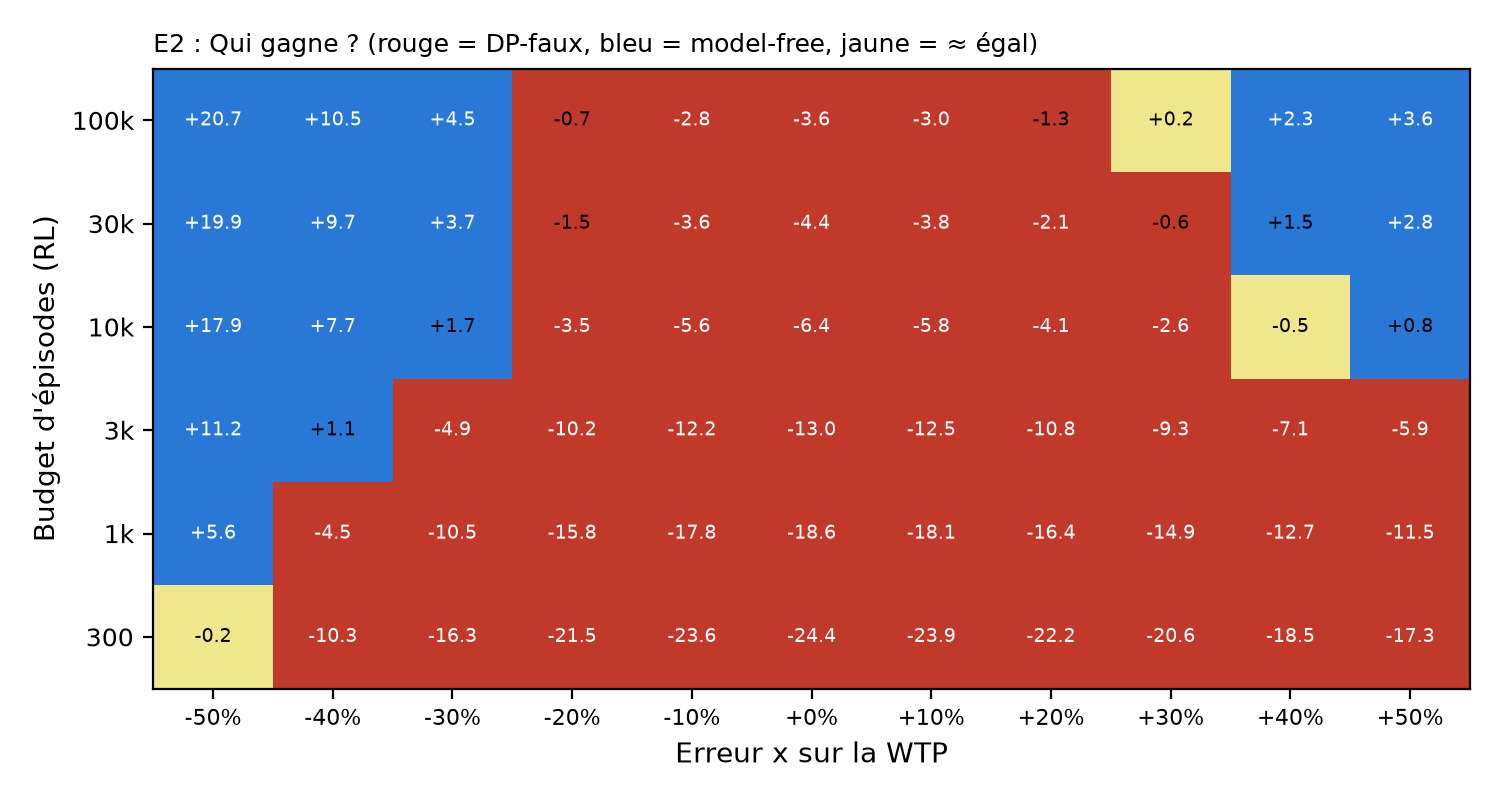
\includegraphics[width=0.85\textwidth]{e2_winner_map.png}
\caption{Carte du vainqueur (E2) : Bleu = RL gagne, Rouge = DP gagne, Jaune = égalité à $\pm 0{,}5\,\%$.}
\label{fig:e2_winner}
\end{figure}

\begin{defbox}[Casquette PROF : L'asymétrie fondamentale de l'erreur]
Pourquoi l'erreur sur la WTP (disposition à payer) produit-elle une telle asymétrie ?
\begin{enumerate}
  \item \textbf{Sous-estimation ($x < 0$) : Le piège mortel.}
  Si la DP croit que la WTP est 50\,\% plus faible qu'en réalité, elle s'affole et propose des prix très bas (50 € ou 80 €) dès les premiers jours ($t > 10$). Les clients loisirs achètent tout, et l'avion se remplit à 88\,\%. Quand arrivent les clients affaires ($t \le 10$) prêts à payer 200 €, \textbf{l'avion est déjà plein}. Le manque à gagner est irréversible. Le revenu s'effondre à \textbf{75,8\,\%}. Le RL bat cette DP dès 1 000 épisodes !
  
  \item \textbf{Surestimation ($x > 0$) : Une erreur pardonnée.}
  Si la DP surestime la WTP de 30\,\%, elle affiche des prix plus élevés. Elle vend moins de sièges aux loisirs, mais conserve son stock intact pour les jours d'affaires. Elle atteint encore \textbf{96,3\,\%} de l'optimum ! Pour la battre, le RL a besoin d'au moins 30 000 à 100 000 épisodes.
\end{enumerate}
\end{defbox}

\begin{tipbox}[Casquette PRÉSENTATEUR : La punchline pour l'oral]
\textit{« Monsieur le professeur, notre résultat central est une asymétrie critique : dans la tarification aérienne, \textbf{être trop pessimiste sur la demande coûte trois fois plus cher qu'être trop optimiste}. Face à un modèle qui sous-estime la clientèle, le Q-learning sans modèle bat la planification dès quelques centaines de vols. Mais face à un modèle modérément optimiste, planifier reste supérieur à l'apprentissage jusqu'à 30 000 épisodes. »}
\end{tipbox}

% ------------------------------------------------------------
\subsection{E3 — Heatmaps des Politiques Apprises}

\begin{figure}[h!]
\centering
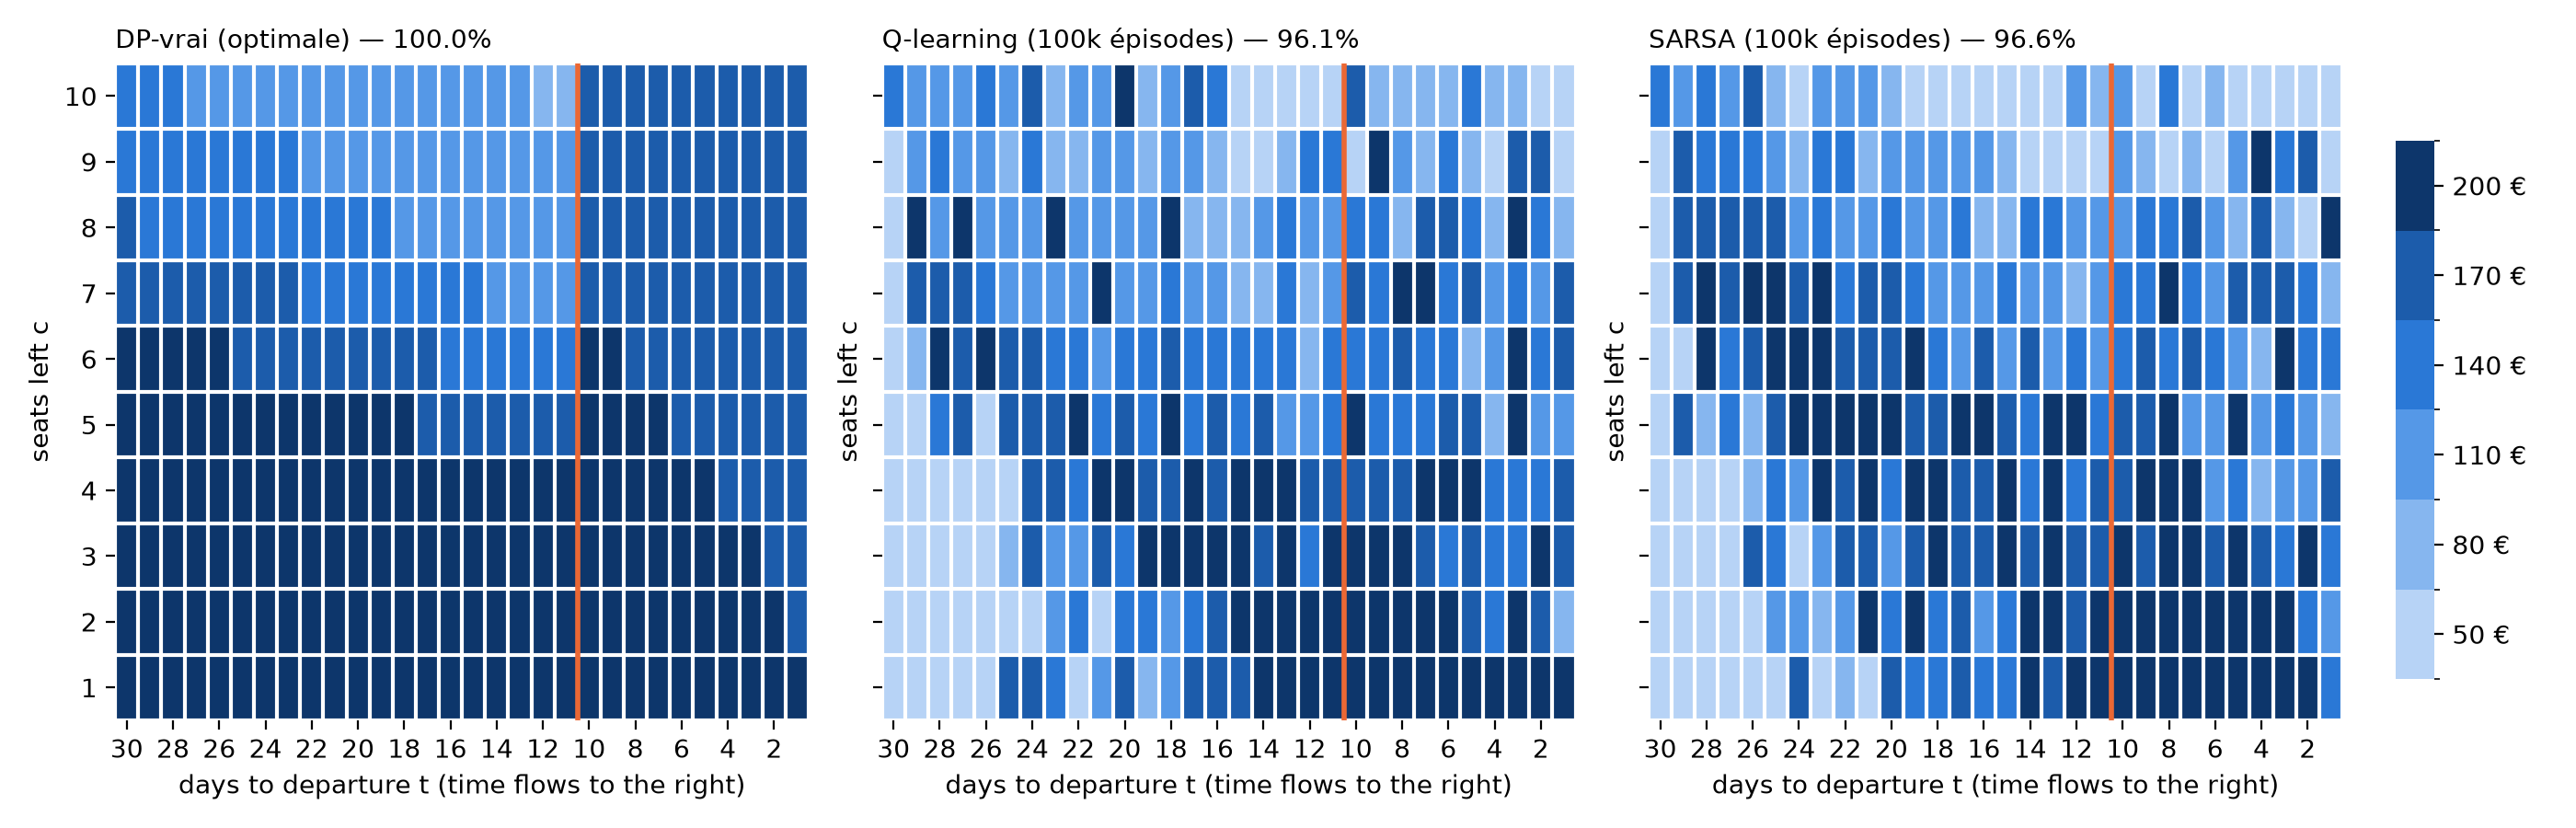
\includegraphics[width=\textwidth]{e3_policy_heatmaps.png}
\caption{Comparaison des politiques : DP-vrai (100\,\%), Q-learning (96,1\,\%), SARSA (96,6\,\%).}
\label{fig:e3_heatmaps}
\end{figure}

L'inspection visuelle des politiques (figure~\ref{fig:e3_heatmaps}) apporte trois enseignements majeurs :
\begin{enumerate}[nosep]
  \item \textbf{La frontière des 10 jours} (ligne orange) : La DP bascule instantanément sur des prix élevés (170--200 €) dès que les clients affaires arrivent ($t \le 10$). Q-learning et SARSA ont parfaitement retrouvé cette règle sans jamais connaître les équations de demande.
  \item \textbf{La protection de l'inventaire} : Quand le nombre de sièges restants $c$ est faible ($c \le 4$), les trois politiques montent les prix dès $t > 10$ pour rationner le stock.
  \item \textbf{Le bruit aux frontières} : Le RL commet des erreurs uniquement dans les états rares (ex. $c=1$ ou $c=2$ à $t=30$ jours, ou $c=10$ à $t=2$ jours), car ces états ne sont presque jamais visités lors des simulations de vols normaux.
\end{enumerate}

% ------------------------------------------------------------
\subsection{E4 — L'effet du facteur d'actualisation $\gamma$ (Myopie)}

Dans un problème à horizon fini ($T=30$), la théorie prescrit $\gamma = 1$. Que se passe-t-il si un ingénieur règle par habitude $\gamma = 0{,}9$ ou $\gamma = 0{,}5$ ?

\begin{figure}[h!]
\centering
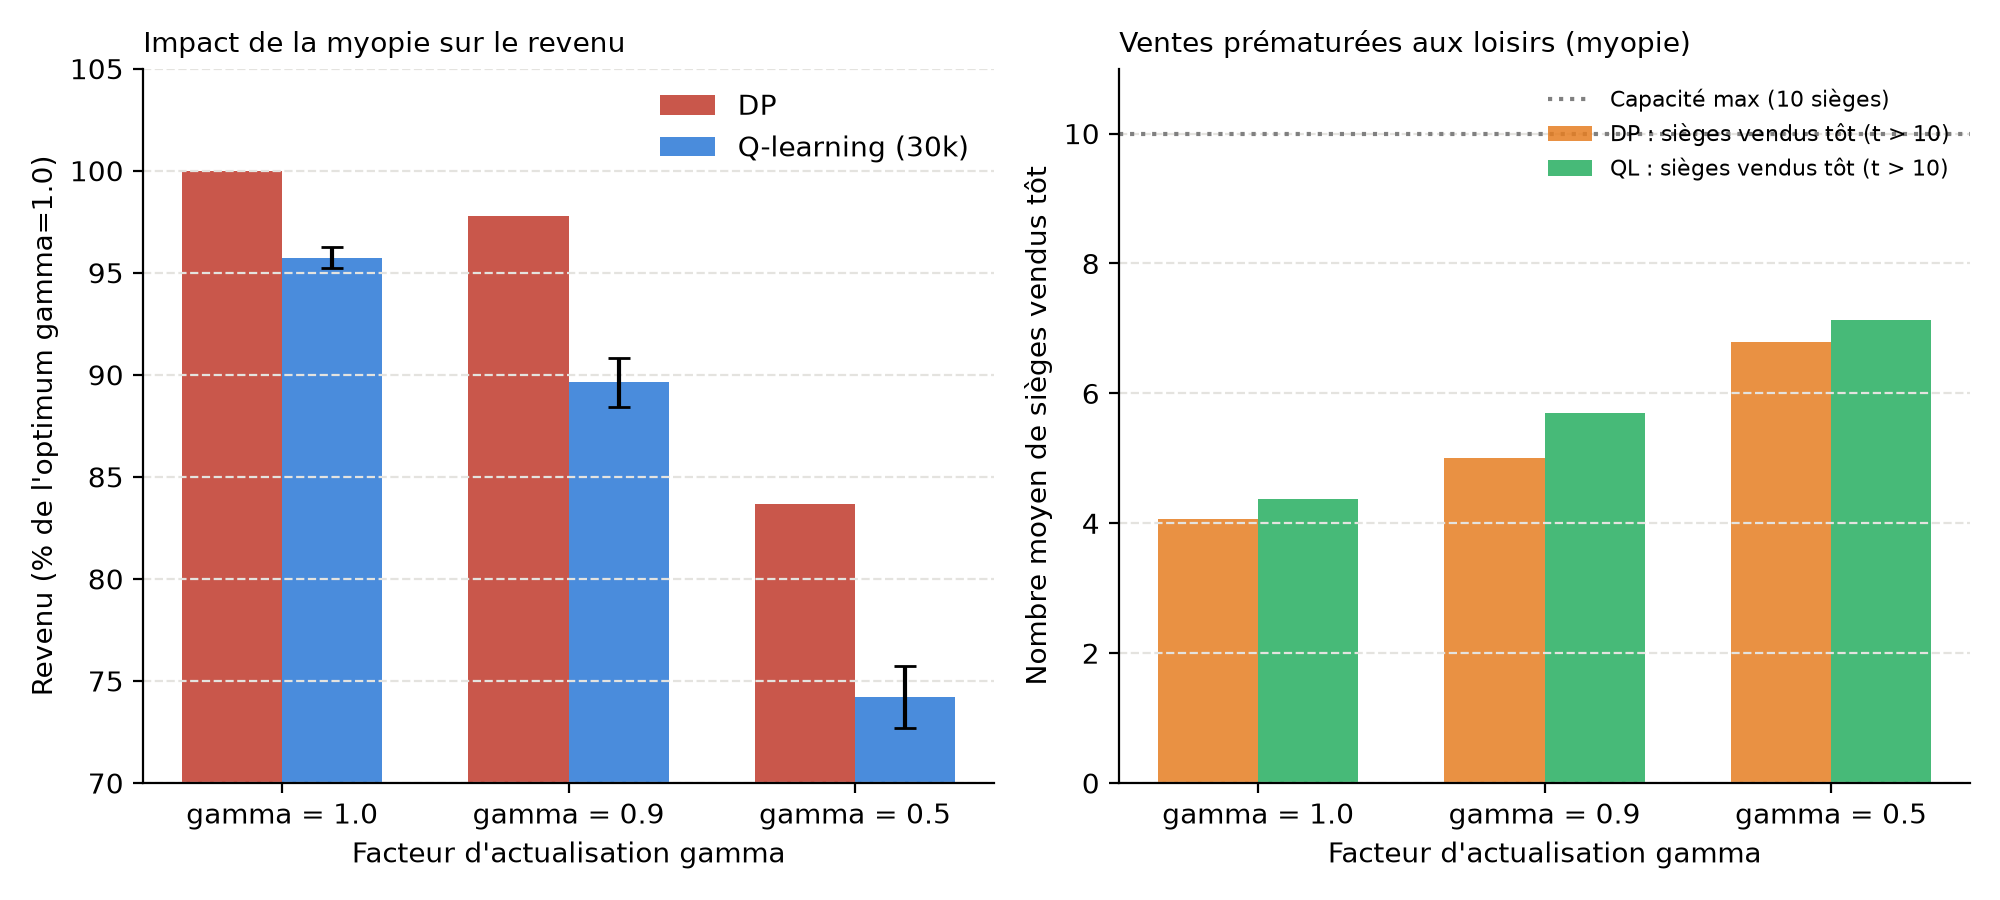
\includegraphics[width=0.85\textwidth]{e4_comparison.png}
\caption{Expérience E4 : Chute de revenu et ventes prématurées quand $\gamma$ diminue.}
\label{fig:e4_gamma}
\end{figure}

\begin{defbox}[Casquette PROF : L'illusion du gain immédiat]
Quand $\gamma < 1$, l'agent déprécie la récompense future : 200 € reçus dans 15 jours ne valent que $200 \times 0{,}5^{15} \approx 0{,}006$ € !
L'agent devient \textbf{impatient} : il préfère encaisser 80 € aujourd'hui plutôt que d'attendre les clients affaires.
Résultat : à $\gamma = 0{,}5$, l'agent vend plus de 7 sièges sur 10 avant le jour 10, provoquant une perte de revenu de 16,3\,\% pour la DP et 21,5\,\% pour le Q-learning.
\end{defbox}

% ------------------------------------------------------------
\subsection{Synthèse pour l'Examen Oral avec Jean Martinet}

\begin{tipbox}[Casquette CHEF DE PROJET : Plan de pitch en 5 minutes chrono]
\begin{enumerate}
  \item \textbf{Minute 1 — Le Problème \& la Question de Recherche} : Présenter le dilemme \textit{Plan or Learn}. Expliquer le MDP (341 états, 6 prix, horizon 30 jours, 10 sièges).
  \item \textbf{Minute 2 — Les Fondations & Cohérence} : Mentionner l'amincissement de Poisson, la récurrence exacte de Bellman pour la DP, et l'évaluation exacte des politiques (56 tests unitaires passants).
  \item \textbf{Minute 3 — Le Crossover (E2)} : Afficher la \textit{Winner Map} ! Souligner l'asymétrie découverte (sous-estimation vs surestimation de la WTP).
  \item \textbf{Minute 4 — Les Politiques Apprises (E1 & E3)} : Montrer les heatmaps. Expliquer pourquoi Q-learning converge plus vite aux budgets moyens et comment Robbins-Monro résout le bruit stochastique.
  \item \textbf{Minute 5 — Conclusion \& Ouverture} : Répondre clairement à la question de recherche et ouvrir vers le Deep RL pour les grands avions ($C=200$).
\end{enumerate}
\end{tipbox}

\end{document}

